\documentclass[11pt,titlepage]{article}
%\usepackage[notref]{showkeys}
\usepackage[reqno]{amsmath}
\usepackage{natbib}
\usepackage{amssymb}
\usepackage{epsfig}
\usepackage{comment}
\usepackage{url}
\usepackage[all]{xy}        
\usepackage{dcolumn}
\newcolumntype{.}{D{.}{.}{-1}}
\newcolumntype{d}[1]{D{.}{.}{#1}}
\usepackage{threeparttable,booktabs}
\usepackage{times}
\usepackage{vmargin}
\setpapersize{USletter}
\topmargin=0in

% Shortcuts
\renewcommand{\P}{\text{P}}
\newcommand{\MC}{\multicolumn}
\usepackage{calc}
\newcounter{hours}\newcounter{minutes}
\newcommand{\printtime}{%
  \setcounter{hours}{\time/60}%
  \setcounter{minutes}{\time-\value{hours}*60}%
  \thehours :\theminutes}
%
\title{Matching as Nonparametric Preprocessing for Reducing Model
  Dependence in Parametric Causal Inference\thanks{Our thanks to Dan
    Carpenter and Jeff Koch for data; Neal Beck, Alexis Diamond,
    Olivia Lau, and Gabe Linz for many helpful comments; and the
    National Institutes of Aging (P01 AG17625-01) and the National
    Science Foundation (SES-0318275, IIS-9874747) for research
    support.  Software to implement the methods in this paper is
    available at \texttt{http://GKing.Harvard.Edu/matchit}.}}

\author{Daniel E. Ho,\thanks{J.D.\ candidate, Yale Law School, Ph.D.\,
    Department of Government, Harvard University. (Center for Basic
    Research in the Social Sciences, 34 Kirkland, Cambridge MA 02138,
    USA; \texttt{http://www.people.fas.harvard.edu/\~\,deho},
    \texttt{daniel.ho@Yale.Edu}).}
%\and %
Kosuke Imai,\thanks{Assistant Professor, Department of Politics, Princeton
    University (Corwin Hall 041, Department of Politics, Princeton
    University, Princeton NJ 08544, USA;
    \texttt{http://www.princeton.edu/\~{}kimai},
    \texttt{kimai@Princeton.Edu}).}
%\and %
Gary King,\thanks{David Florence Professor of Government, Harvard
  University (Center for Basic Research in the Social Sciences, 34
  Kirkland Street, Harvard University, Cambridge MA 02138;
  \texttt{http://GKing.Harvard.Edu}, \texttt{King@Harvard.Edu}, (617)
  495-2027).}
%\and %
Elizabeth A. Stuart\thanks{Researcher, Mathematica Policy Research, Inc.\, Ph.D.\, Department of Statistics,
  Harvard University. (Science Center 702, One Oxford Street,
  Cambridge, MA 02138, USA;
  \texttt{http://www.people.fas.harvard.edu/\~\,estuart},
  \texttt{Stuart@Stat.Harvard.Edu}).}}

\date{\today\ (\printtime)} 
\begin{document}\maketitle

\begin{abstract}
  Although political science articles rarely present causal estimates
  from more than a few model specifications, authors typically choose
  these from numerous trial runs readers never see.  Given the
  typically large variation in estimates across choices of control
  variables, functional forms, and other modeling assumptions, how can
  researchers ensure that the few estimates presented are accurate or
  representative?  How do readers know that political science articles
  are not merely demonstrations that the author found it
  \emph{possible} to find a specification that fits his or her
  favorite hypothesis?  Matching methods, which offer the promise of
  causal inference with fewer assumptions, is one possible way
  forward, but the literature suffers from conflicting approaches to
  estimation, uncertainty, theoretical results, and practical advice.
  We propose a unified perspective on this literature.  Our approach
  makes it possible for researchers to preprocess their data (such as
  with the easy-to-use matching software we offer) and then to apply
  whatever familiar parametric techniques they would have used anyway.
  Instead of replacing existing methods with matching, we use matching
  to make parametric models work better by giving more accurate and
  considerably less model-dependent causal inferences.
\end{abstract}
\baselineskip=1.57\baselineskip

\section{Introduction}

In this paper, we offer procedures to reduce model dependence in
political science research.  Model dependence is a statistical problem
that threatens the validity of a wide variety of quantitative research
in the discipline.  The problem is easy to recognize, but it usually
only arises in private and open discussions of it are rarely found in
the literature.

To see the problem, consider how quantitative political science
research typically proceeds: Even for a single project, we often spend
a year or more collecting, correcting, recollecting, merging, and
recoding data.  When all the data are finally available in the right
format, and loaded into our favorite statistical package, we obtain a
causal estimate by running some parametric statistical procedure ---
linear regression, logit, probit, duration models, structural equation
models, count models, etc.  This run typically takes only a few
seconds and, according to some textbooks, it would be time to write up
the results.

Of course, this never happens.  Instead, we do a second run with
different control variables, a third with a different functional form,
a fourth with a different measure of our key causal variable, one with
different sample periods or observation subsets, and then each of
these or others are repeated with slight variations over and over
again.  Although this usual procedure produces hundreds or thousands
of alternative estimates of our causal effect, we typically only
choose one, and rarely more than 5--10, to present in a paper.  Yet,
we know that our estimates depend on their corresponding modeling
assumptions and that different specifications can yield very different
causal inferences.

The problem for researchers is how to convince readers that we picked
a representative specification or the right one rather than the one
that most supported our favorite hypothesis.  What does it even mean
to choose ``the right'' parametric model estimates when any chosen
model depends on assumptions we cannot verify?  When we read a
published article in political science, how do we know whether the
causal effect presented is accurate or whether the article merely
demonstrates that it was \emph{possible} to find a specification
consistent with the researcher's prior expectations?

We attack this problem by drawing on a new statistics literature on
causal inference based on matching, a nonparametric and
non-model-based statistical procedure.  This work offers considerable
promise for increasing the reliability and validity of causal
inferences by reducing or eliminating the role of functional form and
other assumptions of parametric models.  The statistical literature on
matching has grown theoretically sophisticated, but, from the point of
view of the practical researcher, it looks like a cacophony of
conflicting techniques, practices, conventions, and rules of thumb.
Valid methods for computing standard errors and confidence intervals
are even more complicated, often not used, and sometimes not
available.  Many theoretical results do not apply to practical
applications unless unknown theoretical quantities or specifications
are somehow divined.  Coherent guidelines for practice are
conflicting, absent, or based on clinical experience rather than
scientific evidence or mathematical proof.\footnote{Matching methods
  now comprise a substantial fraction of the empirical work in some
  disciplines, such as epidemiology and medicine.  However, the
  diversity of substantive applications and the conflicting
  methodological languages used to describe the same underlying
  concepts have limited the spread of these powerful techniques to
  much of the social sciences.}

We attempt to reduce model dependence by first unifying this diverse
literature.  In particular, we suggest a procedure by which applied
researchers can make productive use of the ideas developed without
giving up most of their existing analytical strategies.  Our idea is
to use these new nonparametric techniques, not as substitutes for our
present parametric regression techniques, but to make our familiar
parametric techniques work better.  Under our inferential framework,
analysts merely add a simple preprocessing step to their data analysis
procedures.  They then employ whatever statistical models they are
accustomed to using to analyze the preprocessed data rather than the
raw data.  All of the intuition, diagnostics, and knowledge about our
parametric procedures can then be used as before.

Parametric techniques applied to the preprocessed data are typically
far less sensitive to the choices of modeling assumptions than when
applied to the raw data and produce more valid causal inferences.  For
readers, preprocessing is thus good insurance that the author did not
unintentionally cook the books; for investigators, it is a productive
method for finding systematic patterns in our typically noisy data
without having to worry as much about whether unverified modeling
assumptions are correct.  Our preprocessing approach has obvious
advantages in terms of exposition, pedagogy, and ease-of-use, since
our methodology builds on rather than replaces what we have already
learned, brings some order and cohesion to conflicting methodological
literatures, and suggests a relatively straightforward approach for
empirical researchers seeking to make causal inferences.  For example,
our approach suggests a simple, standardized, and valid approach to
computing standard errors and confidence intervals for most of the new
matching techniques.  This strategy also made it possible for us to
write easy-to-use software that implements all the ideas we discuss in
this paper; it is free and available at
\url{http://gking.harvard.edu/matchit}.

Our approach is similar in spirit to \citet{ImaDyk03},
\citet{RosRub84a}, \citet{Rubin79}, and \citet{RubTho00} who each
recommend matching followed by a (different) specific form of
parametric adjustment, as well as intuitively chosen strategies used
in applied research by \citet{Rosenbaum86} and others, as discussed in
\citet{GlaLevMye03}.  It is also similar to \citet{HecIchTod98} who
develop forms of matching combined with semi-parametric (kernel
weighting) analyses, as well as to the parametric bias adjustment for
one form of matching by \citet{AbaImb04} (except that, to avoid
inducing new biases, we recommend below that matching be evaluated
prior to examining the dependent variable, which is not the case with
these latter approaches as generally implemented).  To our knowledge,
the present paper is the first to propose and work out the conditions
for matching as a general method of nonparametric preprocessing,
suitable for improving any parametric method.\footnote{Our idea is
  also similar in spirit to methods in other areas that preprocess
  data so that subsequent analyses can be improved without modifying
  existing techniques, such as multiple imputation
  \citep{Rubin87,KinHonJos01} and outlier and feature detection
  \citep[][Ch.8]{Bishop95}.}

\section{Definition of Causal Effects}

The notation and ideas in this section parallel that in
\citet[][Section 3.1.1]{KinKeoVer94}, but key aspects of it originate
with many others, especially \citet{Rubin74} and \citet{Holland86}.
To explicate these ideas, we use the running example from
\citet[][Section 3.1.1]{KinKeoVer94}, where the goal is to estimate
the electoral advantage of incumbency for Democrats in the U.S.\ House
of Representatives.  The most important idea in this section is that a
causal effect is a theoretical quantity, defined independently of any
empirical method that might be used to estimate it from real data.

The unit of analysis in our example is therefore the congressional
district, which we label with the index $i$ ($i=1,\dots,n$).  In most
of the methodological literature on causal inference, researchers
simplify the exposition by considering only a single dichotomous
causal (or ``treatment'') variable.  We do the same and label it
$t_i$, which takes a value of 1 if unit $i$ receives the treatment and
0 if $i$ is untreated (the ``control condition'').  In our running
example, the treatment is whether the incumbent receives the party's
nomination in district $i$.  Projects with more complicated causal
variables can dichotomize (perhaps in several alternative ways) or use
more complicated methods \citep{ImaDyk03}.  Those with more than one
causal variable of interest can follow all the advice herein for one
variable at a time.

The observed outcome (or ``dependent'') variable is $y_i$, which in
our case is the Democratic proportion of the two-party vote in
congressional district $i$.  Finally, prior to the treatment decision,
each district $i$ has a variety of characteristics, some of which we
measure and collect in a vector denoted $X_i$.  Whether preprocessing
or not, variables that are even in part a consequence of the treatment
variable should never be controlled for when estimating a causal
effect.  This is of course a critical point, since controlling for the
consequences of a causal variable can massively bias a causal
inference; the problem is unfortunately too common in political
science \citep{KinZen04}.

To clarify our inferential goals, we begin by defining the ``realized
causal effect,'' which is the simplest definition available.  To
provide further familiarity with this concept, we briefly show the
close connection between this definition and the goals of the
substantively unrelated but mathematically closely-related missing
data and ecological inference literatures.  We then generalize the
definition to include features of random causal effects that are
useful for understanding connections between nonparametric
preprocessing and parametric models.  Finally, we give specific causal
estimates of interest at the population level.

\paragraph{Realized Causal Effects}
Because of pretreatment differences among the districts (both
measured, $X_i$, and unmeasured), the causal effect may also differ
across the districts.  We therefore define the casual effect at the
district level.

A causal effect is a function of \emph{potential outcomes}: let
$y_i(1)\equiv y_i(t_i=1)$ be the vote we would observe in district $i$
in say the 2008 election if in fact the Democratic incumbent receives
his or her party's nomination (i.e., $t_i=1$), and let $y_i(0)\equiv
y_i(t_i=0)$ be the vote we would observe if the Democratic Party
nominates a nonincumbent (i.e., $t_i=0$).  (Each of the potential vote
outcomes in district $i$ is thus a function of the incumbency status
in the same district, $t_i$, and not a function of candidates in other
districts.)  The use of parentheses in this notation denotes that the
outcome is potential, and so not necessarily observed, and that it
depends on the value of the variable in parentheses.  Since these are
potential outcomes, their values remain the same regardless of whether
the treatment is in fact applied in district $i$ or not.  However, the
key point is that since the Democratic Party either will nominate
($t_i=1$) or will not nominate ($t_i=0$) an incumbent to run in
district $i$, we will observe either $y_{i}(1)$ or $y_{i}(0)$ but not
both.

The difference between the two potential outcomes defines the simplest
realized (or in-sample) definition of a causal effect:
\begin{equation}
  \label{rce}
  \text{(Realized causal effect for unit $i$)} = y_i(1) - y_i(0).
\end{equation}
(This quantity is an unobserved realization of a random variable to be
defined below.)  The fact that one of these potential outcomes is
always a counterfactual --- and thus is never known for certain no
matter how perfect the research design, experimental control, or
number of observations collected --- expresses what is known as the
``fundamental problem of causal inference'' \citep{Holland86}.

\paragraph{Connections to Missing Data and Ecological Inference}
Although causal inference is the ultimate goal of most research
programs in the social sciences, the inherent difficulty of this goal
is not always fully appreciated.  To clarify this issue, and to
further elucidate the definition of causal effects, we now show how
causal inference with observational data is an extreme special case of
two areas of statistics that are widely, but incorrectly, perceived to
be more difficult than causal inference.

If district $i$ receives the treatment, we observe $y_i=y_i(1)$ but
not $y_i(0)$ and otherwise we observe $y_i=y_i(0)$ but not $y_i(1)$.
In this framework, causal inference can be thought of as a severe
missing data problem, where each unit has two relevant dependent
variables, $y_i(0)$ and $y_i(1)$, but one of which, $t_iy_i(0) +
(1-t_i)y_i(1)$, is always missing.  Moreover, since $y_i(0)$ and
$y_i(1)$ are never both observed for any set of units, we cannot use a
known relationship between the two to extrapolate to units where only
one is observed.  Making causal inferences is thus equivalent to an
especially difficult case of imputing missing data, using whatever
external information is available.  As we show below, this connection
will prove useful in making the bridge that connects nonparametric
matching to parametric models.

Causal inference can also be thought of as an especially severe form
of ecological inference.  In ecological inference, we observe for each
observation the proportions representing the two marginals of a
$2\times 2$ contingency table (such as the proportion of people voting
and the proportion of people who are black) and try to estimate the
unknown cell proportions (the proportion of blacks who vote and the
proportion of whites who vote).  To show the connection, we refer to
the known ($y_i$ and $t_i$) and potentially unknown [$y_i(0)$ and
$y_i(1)$] quantities in both problems in the same notation and pay
special attention to the order in which the information is generated:
In both problems, we imagine that $y_i(0)$ and $y_i(1)$ exist in
nature before our research begins.  Then $t_i$ (the treatment in
causal inference or the row marginal in ecological inference) is
applied or otherwise becomes known.  Finally, we can calculate the
observed outcome $y_i$ deterministically via this simple accounting
identity:
\begin{equation}
  \label{id}
  y_i = t_iy_i(1) + (1-t_i)y_i(0).
\end{equation}
In ecological inference, by solving (\ref{id}) for one of the unknowns
as a linear function of the other and recognizing that proportions are
always constrained to the unit interval, we can put deterministic
bounds on both quantities of interest with certainty
\citep[][ch.5]{King97}.  In causal inference, we have the advantage of
always knowing one of the quantities exactly; however, because
(\ref{id}) cannot be solved for one of the unknowns (since it would
require dividing by $t_i$ or $1-t_i$, which includes zero) we have the
severe disadvantage in causal inference of in general not knowing
anything with certainty about the other unknown; this problem does not
arise in ecological inference.

Social scientists correctly think of missing data imputation and
ecological inference as difficult and hazardous areas of statistical
inference.  After all, both involve making inferences about patterns
in unobserved quantities by using patterns in observed data, with
nothing but optimistic assumptions guaranteeing that the former have
anything necessarily to do with the latter.  However, scholars should
be no less concerned when making causal inferences, as every causal
effect ever estimated from observational data involves essentially
identical inferential hazards.  If anything, the specific problems in
making causal inferences are even more difficult than most
applications in these other areas.  Whether using linear regressions,
simple descriptive differences in means, or complicated multiple
equation estimators, causal inference requires assumptions that are no
easier to justify than those in imputation or ecological inference.
In all three areas, the inferential target is not normally highly
constrained by the observed data and so substantive conclusions will
usually depend on unverifiable assumptions about the data generation
process.  Thus, laying these assumptions bare as clearly as possible
throughout the process is essential.

\paragraph{Random Causal Effects} In order to make statistical
inferences, we imagine that the realized potential outcomes in
(\ref{rce}) are realizations of corresponding random variables (for
which we use the corresponding capital letters).  We do not require
that the data are sampled from some specific population, only that
there exists some data generation process that leads to the one
realization we see and could have led to some other realization.  This
logic then produces the random causal effect:
\begin{equation}
  \label{rance}
  \text{(Random Causal Effect for unit $i$)}  = Y_i(1) - Y_i(0),
\end{equation}
features of which we are interested in as alternative quantities of
interest.  For example, our second definition for the causal effect is
the mean causal effect, which is the average over repeated
hypothetical draws of the the random causal effect:
\begin{align}
  \label{meance} \text{(Mean Causal Effect for unit $i$)}
  &= E(\text{Random Causal Effect for unit $i$})\\
  &= E[Y_i(1) - Y_i(0)]\\ \notag &= \mu_i(1) - \mu_i(0),
\end{align}
where $\mu_i(1)\equiv E[Y_i(1)]$ and $\mu_i(0)\equiv E[Y_i(0)]$.

\paragraph{Average Quantities of Interest}
In most applications, we do not attempt to estimate the treatment
effect for each observation, but instead estimate the average over all
observations, for some subset of observations, or for a particular
population or population subgroup.  This leads to several choices for
quantities of interest, each of which is defined for either realized
(in sample) or population causal effects.  We focus on in sample
effects --- i.e., based on quantities of interest for all or a subset
of units in our data --- since they are closer to our data than
effects for averages of specified populations or population subgroups,
but the difference is not always important from a practical viewpoint
since a good estimator for one is ``automatically a good estimator for
the other'' \citep[p.6][]{Imbens04}.

Among in-sample effects, we consider two choices.  The first is the
average treatment effect or ATE:
\begin{align}
  \label{pate}
  \text{ATE} & = \frac{1}{n}\sum_{i=1}^n E[Y_i(1) - Y_i(0)] \notag\\
  &  = \frac{1}{n}\sum_{i=1}^n[\mu_i(1) - \mu_i(0)],
\end{align}
which is the mean causal effect for unit $i$ averaged over all units
(so that the expected value operator in the first line averages over
the random potential outcomes for each unit, and the average over $i$
in both refers to the observed sample).

The alternative choice of a target quantity of interest is the average
treatment effect on the treated, or ATT:
\begin{align}
  \label{att}
  \text{ATT} & = \frac{1}{\sum_{i=1}^n t_i}\sum_{i:t_i=1} E[Y_i(1) - Y_i(0)]\notag\\
  & = \frac{1}{\sum_{i=1}^n t_i}\sum_{i:t_i=1}[\mu_i(1) - \mu_i(0)],
\end{align}
In our running example, this is the average causal effect in districts
in which the Democratic Party nominated the incumbent member of the
House.  From one perspective, we might want to know this treatment
effect on the treated (the ATT) since obviously this is the group of
districts where the treatment was applied.  In other words, the ATT is
the effect of the treatment actually applied.  Medical studies
typically use the ATT as the designated quantity of interest because
they often only care about the causal effect of drugs for patients
that receive or would receive the drugs.  For another example, in job
training programs, we are not normally interested in assigning
employed people to have this training \citep{HecIchTod98}.  In the
social sciences, the ATT is also a reasonable choice, but so is the
average treatment effect (the ATE).  In our running example, we might
be interested not only in the effect of incumbency when the incumbent
is nominated, but we can also imagine what might have happened if an
incumbent were nominated in a district in which he or she did not
actually receive the nomination.  In this paper, we usually focus on
ATT as the quantity of interest when it is conceptually or
algebraically simpler, but we also show how to compute the ATE.

\section{Assumptions and Data Collection Mechanisms}

We now describe the assumptions necessary for making causal inferences
in experimental and observational research.  Some version of these
assumptions, or some way to deal with the information in them, is
necessary no matter what statistical methods are used for estimation.
Any specific statistical method chosen will make additional
assumptions, but the ones discussed here affect essentially all
methods.

\subsection{Experimental}

Although classical randomized experiments are only rarely conducted in
political science, they remain a useful ideal type for understanding
other research designs.  Indeed, some of the assumptions necessary for
valid inference in experiments are approximated by the preprocessing
procedures we suggest below.

Valid and relatively straightforward causal inferences can be achieved
via classical randomized experiments.  Such experiments have three
critical features: (1) \emph{random selection} of units to be observed
from a given population, (2) \emph{random assignment} of values of the
treatment ($t_i$) to each observed unit (in ``classical'' experiments
random assignment is complete and not within fixed clusters or strata
defined by other variables), and (3) a \emph{large $n$}.

The first feature avoids selection bias by identifying a given
population and guaranteeing that the probability of selection from
this population is related to the dependent variable only by random
chance.  Combining this with the large $n$ from the third feature
guarantees that the chance that something will go wrong is vanishingly
small.

Random assignment in the second feature guarantees the absence of
omitted variable bias even without any control variables included.  To
see this, recall that under the usual econometric rules for omitted
variable bias, a variable $X_i$ must be controlled for if it is
causally prior to $t_i$, empirically related to $t_i$, and affects
$y_i$ conditional on $t_i$.
% --- or, in other words, $X_i$ must be
%controlled for if it is correlated with the potential outcomes,
%$y_i(1)$ and $y_i(0)$.  
If instead one or more of the three conditions
do not hold, then $X_i$ may be omitted without any resulting bias
(although the variance may increase).  Random assignment guarantees
that $t_i$ is unrelated to \emph{any} $X_i$, whether measured or not,
except by random chance.  Moreover, the large $n$ condition guarantees
that this chance is vanishingly small.

Classical randomized experiments are a true ideal type, particularly
in relation to most social science research which almost always fails
to meet at least one of the three features.  Even most social science
lab experiments have random assignment but no random selection and
often a small $n$.  Traditional survey research has what is intended
to be random selection (although with dramatically increasing
nonresponse rates and cell phone usage, this is a less plausible
claim) and certainly has a large $n$, but random assignment, except
when the treatment involves the wording of survey questions, is
usually impossible.

\subsection{Observational}

We define observational data collection mechanisms as any process
generating data that does not meet all three features of a randomized
experiment.  Scholars trying to use the experimental paradigm attempt
to design research to meet all three features discussed in the
previous section.  Researchers analyzing observational data are
instead forced to make assumptions that, if correct, help them avoid
various threats to the validity of their causal inferences.

In this paper, we assume data are selected in a manner that does not
generate selection bias.  Observations need not be selected at random,
as in an experiment, but the probability of selection must not be
correlated with the dependent variable $y$ after taking into account
the treatment $t$ and pretreatment covariates, $X$.  Whether this
assumption is satisfied by carefully considering and controlling for
the sample selection process or by changing the quantity of interest
to be that reflected by the sample, avoiding selection bias is not a
trivial matter, and indeed is the subject of a great deal of concern
and study in a large variety of methodological and substantive
literatures.  We mention it here to emphasize that all the well-known
concerns about selecting on the dependent variable should remain a
concern to researchers even when adopting our approach of
preprocessing data via nonparametric matching procedures.

We also assume that a researcher analyzing observational data has
sufficient information in their measured pretreatment control
variables $X$ so that it is possible via \emph{some} method to make
valid causal inferences.  This is known in some fields as the absence
of omitted variable bias, so that $X_i$ must include all variables
that are causally prior to $t_i$, associated with $t_i$, and affect
$Y_i$ conditional on $t_i$ \citep{Goldberger91,KinKeoVer94}.  In other
fields, this same condition is known as ignorability, which means that
$t_i$ and the potential outcomes are independent after conditioning on
$X_i$, and so we can literally ignore all unobserved variables
\citep{RosRub83}.  Ignorability is a strong condition, but it is one
about which social scientists are deeply knowledgeable and which is
the central methodological concern of many substantive scholarly
articles.  We emphasize this assumption to make clear that our
procedures contain no magic: They are unable to control for variables
that are not measured.

In the context of the no selection or omitted variable bias
assumptions, we have implicitly made three others that are worth
additional emphasis here.  First, pretreatment covariates $X$ are
truly pretreatment and are thus not consequences of $t$.  Second, we
assume the independence of units, which is the equivalent of assuming
the absence of time series or spatial autocorrelation (or in other
words that the two potential outcomes for observation $i$ and the
treatment for observation $j$ are independent, for all $i\not=j$).  We
have also assumed that all treatments are the same.  This assumption
would be violated in our running example if incumbency status meant
something different across districts.\footnote{These last two
  assumptions are sometimes known under the awkward name of the
  ``stable unit treatment value assumption'' or SUTVA
  \citep{Rubin74}.}

Satisfying the assumptions discussed in this section still leaves many
other assumptions to be made when choosing a specific statistical
inference method.  We now focus on this point in the context of
commonly used parametric methods.

\section{Parametric Analysis Methods}

Researchers willing to assume that a particular parametric model (up
to some unknown parameters) generated their data should specify and
directly estimate this model.  Preprocessing data with matching
procedures is suboptimal in this situation.  Of course, few
researchers with real observational data sets have this kind of
knowledge and as a result some choices need to be made among the range
of possible parametric models.  The dilemma then is that although
researchers using parametric methods do not know the true parametric
model, they must proceed as if they do.

We begin to elaborate this problem and some paths forward by
specifying a single but general parametric model that characterizes
the range of models that researchers might choose from.  The special
cases of this model include almost all parametric models that have
been used in the social sciences.  First, define the chosen stochastic
component for the model as $Y_i \sim p(\mu_i,\theta)$ for probability
density $p(\cdot)$, mean $\mu_i$, and vector of ancillary parameters
$\theta$.  Then, denote the systematic component as $\mu_i\equiv
E(Y_i|t_i,X_i)=g(\alpha + t_i\beta + X_i\gamma)$ for some specified
functional form $g(\cdot)$ and with intercept $\alpha$ and
coefficients $\beta$ and $\gamma$.  The ancillary parameters may also
be specified to vary over observations as a function of $X_i$ or other
covariates.  This framework includes all generalized linear models
\citep{McCNel89}, as well as many others.  For example, if $p(\cdot)$
is normal and $g(c)=c$, we have linear regression; if $p(\cdot)$ is
Bernoulli and $g(c)=1/(1+e^{-c})$, the model reduces to a logistic
regression.

We define the ATT in equation~(\ref{att}) under this model by plugging
in the definitions of the potential outcomes from the systematic
component, with $t_i$ taking on values 1 and 0 respectively:
\begin{align}
  \label{matt}
\mu_i(1)&\equiv E(Y_i(1)|t_i=1,X)= g(\alpha + \beta + X_i\gamma),\notag \\
\mu_i(0)&\equiv E(Y_i(0)|t_i=0,X) = g(\alpha + X_i\gamma).
\end{align}
We can produce estimates of these quantities by assuming independence
over observations, and forming a likelihood function
\begin{equation}
  \label{lik}
  L(\alpha,\beta,\gamma,\theta|y, t, X) = \prod_{i=1}^n 
  p\left(y_i \mid g(\alpha + t_i\beta + X_i\gamma), \theta\right),
\end{equation}
the maximum of which gives parameter estimates.

We now turn to the difficulties in making causal inferences from
experimental vs.\ observational data under this general model.

\subsection{Experimental Data}\label{s:paraexp}

In experimental data, random assignment guarantees (among other
things) that $T$ and (any observed or unobserved) $X$ are independent.
In this situation, $X$ cannot be a confounding factor when estimating
the effect of $T$ and so we drop $X$ and simplify
Equation~(\ref{matt}) as
\begin{align}
  \label{smatt}
  E[Y_i(1)|t_i=1] &\equiv \mu_i(1) = g(\alpha + \beta)\notag \\
  E[Y_i(0)|t_i=0] &\equiv \mu_i(0) = g(\alpha)
\end{align}
and the average treatment effect on the treated in
Equation~(\ref{att}) as
\begin{equation}
  \label{satt}
  \text{ATT} = g(\alpha+\beta) - g(\alpha),
\end{equation}
which importantly no longer has a summation sign over $i$.

The systematic components in equations~(\ref{smatt}) are now scalar
constants for all $i$.  This is a key result, since it means that
changing the definition of the functional form $g(\cdot)$ no longer
models a high dimensional space representing how the mean varies over
$i$ as a function of all the variables in $X$, but insteads now merely
amounts to nothing more than a simple scalar reparameterization.  The
fact that $g(\cdot)$ is now a scalar is central: Since maximum
likelihood is invariant to reparameterization --- meaning, for
example, that the MLE of $\alpha$ is the same as the square root of
the MLE of $\alpha^2$ \citep[][p.75--76]{King89} --- we get the same
estimate of the expected potential outcomes no matter how $g(\cdot)$
is defined.\footnote{To rule out degenerate cases such as $g(a)=8$, we
  require that the image of $g(\cdot)$ and the range of the potential
  outcomes be the same.}  Thus, when $\mu$ is a function of $X$, the
choice of $g(\cdot)$ is a difficult substantive decision typically
requiring more knowledge than is available.  In contrast, in
experimental data, because we can now drop $X$, the choice of
$g(\cdot)$ reduces to an easy computational issue with no substantive
import.  Moreover, given any chosen stochastic component, this result
holds for a wide range of parametric models, including all the special
cases of the general model given above.

Since the specific maximum likelihood estimator of the population mean
for many of common probability densities is merely the sample mean,
the analysis of classical randomized experiments often comes down to
taking the difference in the sample means of $y$ for the treatment and
control groups.  But even if one chooses to run a parametric model
(for reasons of efficiency, conducting conditional inferences, or
because of knowledge of the functional form), the absence of model
dependence means that the choice for a functional form will not
matter: The results will be almost the same no matter what choice one
makes for the functional form.

\subsection{Observational Data} \label{s:paraobs}

In experiments, random assignment breaks the link between $T$ and $X$
and, by so doing, eliminates the problem of model dependence.  When
analyzing observational data with parametric methods we are not so
fortunate.  We cannot reduce equations~(\ref{matt}) to
equations~(\ref{smatt}) and so are left having to model the full
functional relationship that connects the mean as it varies as a
function of $t$ and $X$ over observations.  Since $X$ is typically
multidimensional, this is a surprisingly difficult task with rather
severe consequences for research practice.

The problem is the curse of dimensionality and the consequence in
practice is model dependence.  We begin with the former and for
simplicity suppose that we have a dependent variable and one
ten-category explanatory variable, and our goal is to use linear
regression technology to estimate the functional relationship without
actually making functional form assumptions.  To do this, we represent
the ten categories with ten parameters (a constant and nine dummy
variables or equivalently 10 mean indicator variables).  In contrast,
the usual approach to estimation is to assume linearity by directly
including the ten-category variable.  This enables us to enter not 10
indicator variables, but rather only a constant term and one slope
coefficient.  How do we get from ten parameters to only two?  Pure
assumption.  If we have some sense that the relationship is indeed
linear or close to linear, this is a good use of external information
to reduce the number of parameters that must be estimated.  If not,
then we still have the best {\it linear} approximation to the
conditional expectation function, but the relationship we estimate can
be far off.  If we are running this regression for the purpose of
estimating a causal effect, then the treatment variable is also in the
regression, and its coefficient can be biased to any degree if the
functional relationship with the control variables is misspecified.

This problem quickly becomes more serious as the number of explanatory
variables increases.  For example, estimation without functional form
assumptions with two ten-category explanatory variables would require
not 20 parameters but 100.  In this case, the usual approach would
include a constant term and two slope coefficients, reducing 100
parameters to three by pure assumption.  And with multiple explanatory
variables, claims about external knowledge constraining the functional
form much become dubious.  In this example, by what theory would we
know that 97 parameters, representing every form of nonlinearity and
interaction, should be set to exactly zero?  Including a linear
interaction would not help much since it would merely add one more
parameter to estimate, and so we would still need to make assumptions
about the remaining 96 parameters.

The problem escalates very fast as the number of explanatory variables
increases.  With $V$ 10-category variables, we need $10^V$ parameters
for estimation in a regression framework without functional form
assumptions.  So five explanatory variables leads to a regression
model with 100,000 parameters, and the usual approach works by
estimating only a constant term and five slope coefficients and
restricting by assumption the remaining 99,994 parameters.  Nine such
explanatory variables leaves us with a model with one \emph{billion}
parameters, to be approximated by only the ten that we would estimate
under the traditional approach.  Eighty ten-category explanatory
variables would require a regression model with more parameters than
the estimated number of elementary particles in the universe.

Estimating rather than making assumptions about all these extra
parameters is obviously not possible under the standard regression
approach, since social science data sets do not come with anywhere
near enough observations.  We cannot avoid the problem with nonlinear
or non-normal statistical models, since these pose the same curse of
dimensionality as linear regression.  The assumption of ignorability,
which enables us to make the positivist assumption that we have
measured and observe all necessary variables, is insufficient.

Instead, we are led to the inescapable conclusion that, in parametric
causal inference of observational data, many assumptions about many
parameters are frequently necessary, and only rarely do we have
sufficient external information to make these assumptions based on
genuine knowledge.  The frequent, unavoidable consequence is high
levels of model dependence, with no good reason to choose one set of
assumptions over another.  Residual and other diagnostics will uncover
some forms of misspecification, but the curse of dimensionality
prevents any simple parametric solution to the problem.

To illustrate the problem of sensitivity to model specification, the
left graph of Figure~\ref{fg:extrap} plots artificial data for outcome
$Y$ on the vertical axis and a pretreatment covariate $X$ on the
horizontal axis.  Each data point is plotted as a ``T'' for treated
units ($t_i=1$) and ``C'' for control units ($t_i=0$).  We then fit
two regressions to these data.  The first is a linear regression of
$Y$ on a constant, $X$, and $t$: $E(Y_i|X_i,t_i)=\alpha + t_i\beta +
X_i\gamma$.  The fitted values for this graph are portrayed in two
parallel solid lines, the dark solid line for the treated group,
$E(Y_i|X_i,t_i=1)=\alpha+\beta+X_i\gamma$, and the gray solid line is
for the controls, $E(Y_i|X_i,t_i=0)=\alpha+X_i\gamma$. The small but
positive vertical distance between the two straight lines is this
parametric model's causal effect estimate.
\begin{figure}[t] 
 \begin{center}
   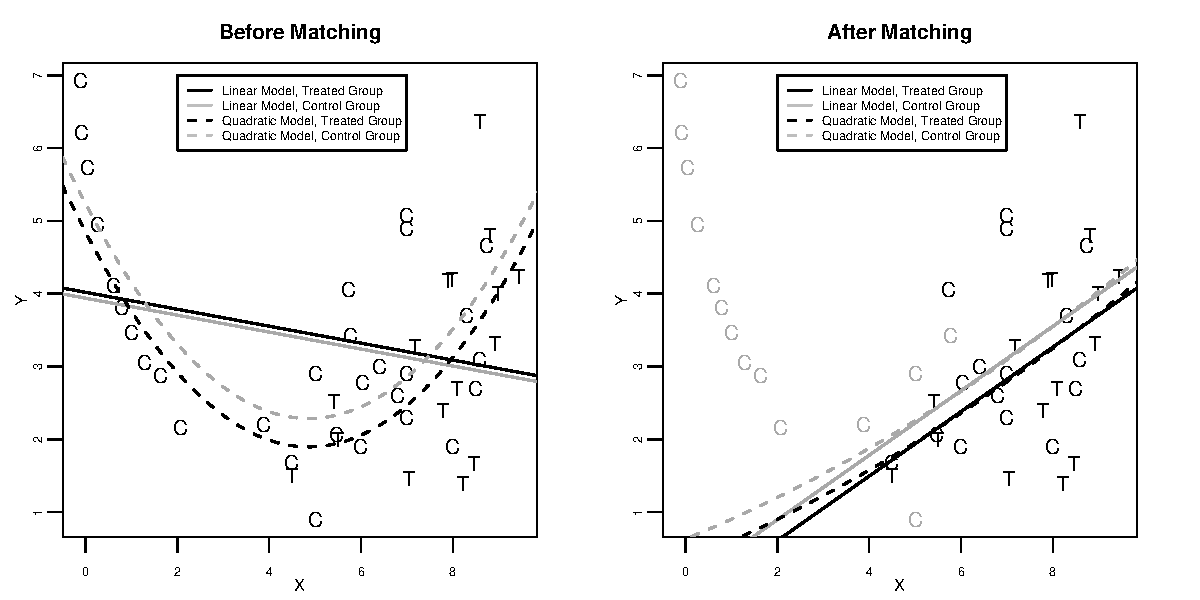
\includegraphics[width=6in]{figs/olspanel-thick.pdf}
  \end{center}
  \vspace{-0.275in}
  \caption{Model sensitivity of average treatment effect estimates for
    imbalanced raw and balanced matched data.  This figure presents an
    artificial data set of treated units represented by ``T'' and
    control units represented by ``C.'' The vertical axis plots $Y$
    and the horizontal axis plots $X$.  The panels depict estimates of
    the average treatment effect for a linear and quadratic
    specification, represented by the difference between parallel
    lines and parabolas, respectively.  Dark lines are fitted to the
    treated points and gray to the controls.  In the raw data, plotted
    in the left panel, the models must extrapolate for treated units
    with $X$ values below 4 and are therefore highly sensitive to
    specification.  In the matched data, plotted in the right panel,
    treated units are matched with control units that are close in $X$
    (gray units are discarded) and as a result treatment effect
    estimates are similar regardless of model specification.}
  \label{fg:extrap}
\end{figure}

Model dependence is easy to see by also fitting a quadratic model to
the same data, which merely involves adding an $X^2$ term to the
original linear regression.  Fitted values for the quadratic
regression appear as dashed curves in the same left graph, again gray
for the controls and solid black for the treated.  Clearly, these fit
the same data markedly differently from the original regression.  Not
only is the overall shape completely different, but the causal effect
has now switched signs and become much larger (this can be seen in the
graph because the gray solid line is slightly below the dark solid
line, whereas the gray dashed curve is substantially above the dark
dashed curve).

Ultimately, these two models estimate the causal effect by the average
vertical distance between the C's and T's.  They differ only in how
they compute this average.  The key problem that generates model
dependence is the absence of any treated unit values with $X$ less
than 4.  This means that to estimate features of $Y(1)$ on the left
side of the graph requires extrapolation over a considerable distance
from where the T's are observed.  These extrapolations make causal
effect estimates exquisitely sensitive to minor modifications in the
statistical model.  In other words, in parametric analyses, the curse
of dimensionality requires a large number of assumptions to which
estimates may be sensitive.  And ``unbalanced'' data like these
require extrapolation, which means that different assumptions will
produce different estimates.

Some researchers surely respond to this diversity of possible models
by inadvertently choosing specifications that support their favored
hypotheses.  Current best practice is to portray forthrightly at least
some aspects of specification uncertainty in published work by giving
results for multiple specifications and evaluating how model dependent
the substantive results are.  But researchers of course do not often
go very far in portraying the sensitivity of their causal inferences
to model specification, and conveying all the sensitivity is
essentially impossible.  Indeed, attempts to do so in many situations
lead to nihilistic conclusions.\footnote{Two approaches to this
  problem include extreme bounds analysis \citep{Leamer78}, which is a
  somewhat standardized way to portray model dependence, and Bayesian
  model averaging \citep{HoeMadRaf99,ImaKin04}, which is intended to
  draw inferences by appropriately combining inferences from models
  with different specifications.}

\section{Nonparametric Preprocessing} \label{s:nonparpreproc}

The goal of matching in general and our specific nonparametric
preprocessing approach in particular is to adjust the data prior to
the parametric analysis so that (1) the relationship between $t_i$ and
$X_i$ is eliminated or reduced, and (2) no bias and little
inefficiency is induced.  If we are able to adjust the data so that
$t_i$ and $X_i$ are completely unrelated (which makes the control and
treatment groups are identical with respect to $X$), we will have
moved a good deal of the way from Section \ref{s:paraobs} to Section
\ref{s:paraexp}.  An assumption of ignorability is still necessary,
but we would no longer need to model the full parametric relationship
between the dependent variable and the multidimensional $X_i$.  This
also eliminates an important source of model dependence in the
resulting parametric analysis stemming from the functional form
specification and the curse of dimensionality.  For data sets where
preprocessing reduces the extent of the relationship between $t_i$ and
$X_i$, but is unable to make them completely independent, model
dependence is not eliminated but will normally be greatly reduced.
Indeed, if nonparametric preprocessing results in no reduction of
model dependence, then it is likely that the data have little
information to support causal inferences by any method, which of
course would also be useful information.

But how can we adjust the data without inducing bias in our causal
estimates?  The key to this problem is that the fundamental rule for
avoiding selection bias --- not selecting on the dependent variable
--- does not prevent us from selecting observations on the explanatory
variables ($t_i$ or $X_i$).  (Random or other physical assignments in
experiments by the investigator and stratified sampling in surveys are
examples of valid data collection mechanisms that select observations
given chosen values of the explanatory variables.)  We can also
select, duplicate, or selectively drop observations from an existing
sample without bias, as long as we do so using a rule that is a
function only of $t_i$ and $X_i$.  Our preprocessed dataset will
therefore include a selected subset of the observed sample for which
$t_i$ and $X_i$ are unrelated, meaning that the treatment and control
groups have the same background characteristics, or in other words
that this relationship holds:
\begin{equation}
  \label{balance}
  p(X|t=1) = p(X|t=0).
\end{equation}

The simplest way to satisfy equation~(\ref{balance}) by preprocessing
is to use \emph{one-to-one exact matching}.  The idea is to match each
treated unit with one control unit for which the values of $X_i$ are
identical.  Our preprocessed dataset thus is the same as the original
dataset with any unmatched units discarded, with $t_i$ and $X_i$ now
independent.  If enough matches are available, this procedure
eliminates all dependence on the functional form in the parametric
analysis.  It is also highly intuitive, since it directly parallels an
experiment where we find pairs of units that are identical in all
observable ways and assign one from each pair to be treated and the
other to be a control.  Then no matter what effect $X_i$ has on $y$,
we can ignore it entirely since $X_i$ is literally held constant
within each pair of units.

Although one-to-one exact matching can eliminate model dependence and
any bias from incorrect assumptions made during the parametric stage
of analysis, it has the disadvantage in many applications of not
generating many matches.  The problem is most severe if $X_i$ is high
dimensional (another effect of the curse of dimensionality) or
contains continuous variables.  The result may then be a preprocessed
data set with very few observations that results in a parametric
analysis with large standard errors.  In this situation, we may reduce
model dependence and the potential for bias, but decrease efficiency
and as a result increase mean square error.  If this occurs in
practice, those in the matching literature tend to sacrifice some bias
reduction for the increased efficiency that comes from having more
observations in the preprocessed dataset.  In our approach, if we lose
some opportunity for bias reduction we do so only in the preprocessing
stage; our second stage parametric analysis still has a chance to
eliminate the remaining bias.  We therefore now turn in Section
\ref{s:choose} to a menu of matching procedures that enable
researchers to satisfy equation~(\ref{balance}) as closely as possible
while still generating a preprocessed dataset with enough
observations.

Finally, the right graph in Figure \ref{fg:extrap} gives an example of
the consequences for reducing model dependence of matching that is not
exact.  The data in this panel is the same as that for which the
parametric analyses in the left graph give highly model dependent
results.  The difference is that the matching procedure deleted the
observations that would require substantial extrapolation (marked as
gray C's).  With these deletions, the data set is now highly balanced,
and as such the linear model and the quadratic model give almost
identical causal effects.  Preprocessing has therefore made the
assumption about whether to include $X^2$ in the regression largely
irrelevant.  Indeed, for a large range of models, this preprocessed
data will be mostly insensitive to the choice of functional form
assumptions and so will return highly similar causal effect estimates.

\section{Choosing a Matching Procedure}\label{s:choose}

In this section, we offer a step by step guide for navigating the wide
variety of matching procedures proposed throughout the statistics,
economics, epidemiology, medical, and biostatistics literatures.
These are young and fast-growing areas, and so we try to distill the
current collective wisdom when one is available or, when not, to
suggest an approach that is at least widely recognized as reasonable.
For detailed reviews of the technical literatures, and other matching
procedures, see \citet{Imbens04}, \citet{Rosenbaum02}, and
\citet{Stuart04} and the detailed user's guide to the software that
accompanies this paper (see Appendix \ref{s:matchit}).

The goal of matching is to improve \emph{balance}, the degree to which
the treatment and control $X$ distributions resemble each other,
without losing too many observations in the process.  The main
diagnostic of success is also balance (as well as the number of
observations remaining).  We judge balance at first by taking the
difference in the treatment and control group means or full histograms
for each variable in $X$.  These can be supplemented by comparing the
means of the squares and cross-products of the variables and higher
order moments or with more dimensions.

In our quest for better balance, one can try any number of matching
procedures, with the final preprocessed data set the one with the best
balance.  To ensure that selection during preprocessing is only on $X$
(to prevent inducing bias), the outcome variable $y$ should not be
examined during the preprocessing stage.  As long as $y$ is not
consulted, preprocessing cannot result in stacking the deck one way or
another.  Experimentalists typically follow a similar procedure by
repeating randomization as often as desired before collecting the
outcome data.  Thus, if an undesirable randomization is obtained, such
as with all men in the treated group and all women in the control
group, they merely discard the first randomization and do it again
until better data are obtained \citep[see][]{Rubin01}.

We recommend four steps of preprocessing, followed by standard
parametric modeling of the preprocessed data set.  We describe this
procedure for the ATT, and so the matching is designed to choose
control units that look most like the treated units.

\paragraph{1. Select Covariates}  
Include all variables in $X$ that would have been included in your
parametric model without preprocessing.  By the usual rules for
avoiding omitted variable bias these should include all variables that
may affect the treatment assignment and the dependent variable.
Including variables only weakly related to treatment assignment will
usually reduce bias more than they will increase variance when using
matching and so most should normally be included \citep{RubTho96,
  HecIchSmi98}.  To avoid post-treatment bias, exclude variables
affected by the treatment variable
\citep{FraRub02,Greenland03,KinZen04}.

If all the variables in $X_i$ are categorical, try exact matching in
Step 2.  Otherwise, try propensity score matching in Step 3.
\paragraph{2. Try Exact Matching}  
Match each treated unit to all control units with exactly the same
covariate values.  This procedure is more general than one-to-one
matching, since we use as many control units as are available for each
treated unit.

If a large number of units were matched, then we have exact balance
with little inefficiency and we may skip the remaining steps and
proceed to the parametric analysis.  If insufficient matches are
found, either repeat the exact matching with fewer covariates or
switch to propensity score matching, described in Step 3.  In the
former, we balance the included variables but do not balance at all on
the rest.  The excluded variables may be partially balanced due to
correlations with the included variables, but some balance will be
absent.  In contrast, propensity score matching uses all variables
but only approximately matches.

\paragraph{3. Use Propensity Score Matching}  
The first step in this procedure is to summarize all the variables in
$X$ with a single variable called the \emph{propensity score}
\citep{RosRub83}.  The propensity score is the true probability of
unit $i$ receiving treatment, given the covariates $X_i$, $e_i(X_i) =
P(T_i=1 | X_i)$.  It is usually estimated via a logistic regression of
$t_i$ on a constant term and $X_i$ (still without regard to the
dependent variable).  The propensity score is central to modern
matching methods, but the present state of statistical theory means
that its role as a theoretical idea differs profoundly from its role
in practice.  Understanding this disconnect, an explanation of which
to our knowledge has not explicitly appeared before in the literature,
is fundamental to making good practical use of this important concept.

Theoretically, the true propensity score is valuable because it is a
``balancing score,'' meaning that if a group of units have similar
propensity score distributions, then the covariates will be balanced
in the treated and control groups on all variables in $X$.  In
addition, if the treatment assignment is ignorable given the
covariates $X_i$, then it is also ignorable given only the propensity
score.  This means that matching can be done using just the
one-dimensional propensity score, instead of all of the covariates
$X$.  Using the true propensity score in this way thus would seem to
solve the curse of dimensionality for matching.

In practice, however, we do not know the true propensity score (except
perhaps in unusual situations).  We would still be able to appeal to
the true propensity score's theoretical properties if we had a
consistent estimate of it, but such an estimate would require knowing
the correct functional form for the assignment model, which is highly
unlikely.  Moreover, few useful theoretical results exist for the case
when the true form of the propensity score equation remains unknown.
These theoretical results would therefore seem to be entirely
self-defeating: In order to use nonparametric matching to avoid
parametric modeling assumptions, we must know the parametric
functional form of the propensity score equation!

Fortunately, there is a way out.  We suggest, first, looking past the
theoretical properties of the propensity score, except for the purpose
of motivating the goal of better propensity score specification, and
second and more importantly, recognizing the value of what we call the
\emph{propensity score tautology}.  The propensity score tautology in
our view is the main justification for using this technology in
practice: The estimated propensity score is a balancing score when we
have a consistent estimate of the true propensity score.  We know we
have a consistent estimate of the propensity score when matching on
the propensity score balances the raw covariates.  Of course, once we
have balance on the covariates, we're done and don't need to look
back.  That is, it works when it works, and when it doesn't work, it
doesn't work.

The tautology thus provides a way to make irrelevant the knowledge of
whether we have satisfied the conditions necessary to use the
theoretical results about the true or consistently estimated score.
The goal of matching is to achieve the best balance for a large number
of observations, using any method of matching that is a function of
$X$, so long as we do not consult $y$.  As it turns out, and for
whatever reason, one such method that researchers have found useful in
a diverse array of applications is based on propensity scores.  The
reason the propensity score approach often works in practice to
balance the covariates relatively quickly may be related to the
theoretical properties of the true score discussed above, but this
conjecture is both unproven and irrelevant to making valid causal
inferences.  At least given the current state of the literature, only
this practical advice based on the propensity score tautology is
useful in practice.

In applications, the usual practice is to estimate the propensity
score by a logistic regression of $t_i$ on $X_i$ and a constant term.
Since we are in the situation where exact matching is insufficient, we
match each treated unit to the control unit with the most similar
value of the estimated propensity score $\hat{e}_i$ (which is known as
nearest neighbor matching on the propensity score).  If this procedure
balances $X$ (and thus satisfies the procedures for checking balance
we describe in Step 4), we use it.  If not, then we respecify the
logistic regression by adding interactions or squared terms and match
again.  If that works, then we use it.  If not, we can try even more
elaborate specifications (when necessary, perhaps even trying other
functional forms such as CART, neural network analyses, or others).

The collective wisdom of the literature also recommends four more
specific rules for applying propensity scores.  First, if many more
control than treatment units are available, consider choosing more
than one control match for each treated unit.  This will increase the
efficiency of the procedure (although each match past the first
usually reduces the variance somewhat less than the previous one).
If, instead, fewer controls are available than those treated, then
matching with replacement --- allowing each control unit to be matched
to more than one treated unit --- is a good option.  Alternatively,
consider switching the definition of treatment and control groups
(although, of course, if using ATT, this will change the substantive
definition of the causal effect).

Second, we are sometimes in the situation of suspecting from prior
evidence (but not from the present data set) that a small number of
covariates have a disproportionately large effect on our outcome
variable.  When this is the case, even slightly mismatching on these
variables may severely bias our causal effect.  To avoid this problem,
we match using two separate metrics, one for the large-effect
variables and another for the rest.  If feasible, we create pools of
exact matches on the large-effect variables and then use nearest
neighbor propensity score matching based on the remaining variables to
choose specific matches within these pools.  If exact matching does
not turn up sufficient observations, then we can choose the nearest
neighbor on the large-effect variables, defined by the Mahalanobis
distance, among all units within 0.25 standard deviations (also known
as ``calipers'') of the propensity score computed from all other
variables.\footnote{The 0.25 standard deviation figure, which is the
  most common recommendation in the literature, appears to be
  interpolated from the results in \citet{CocRub73}.  The Mahalanobis
  distance is the weighted average of the squared distance between
  units $i$ and $j$, $(X_i-X_j)'\Sigma^{-1}(X_i-X_j)$, where $\Sigma$
  is the sample variance matrix of $X$ in the control group.  See
  \cite{RubTho00}.}

Third, if some control units fall outside the range of the treated
propensity score values, then these controls cannot be adjusted to
match the treated units without extrapolation.  Common practice is to
discard these control units.  Similarly, if any treated units fall
outside the propensity score range of the control units, these too are
discarded.  Dropping treated units changes the causal effect being
estimated, but if it remains a relevant quantity, at least it can be
estimated in a reasonable way.  Discarding these nonoverlapping
observations eliminates the need for extrapolation.

Finally, if finding a matching procedure with good balance and a large
number of observations is otherwise difficult, use subclassification.
To use this procedure, divide the units into roughly equally sized
subclasses where the propensity score is, by construction,
approximately constant, and thus balanced.  Generally five or six
subclasses are sufficient to adjust for a univariate covariate such as
the propensity score \citep{Cochran68,RosRub84}.  If balance is
achieved with a reasonable number of observations within each
subclass, then the analysis procedure is carried out within each
subclass and the results are averaged.

\paragraph{4. Evaluate the Matching Procedure}
A good matching procedure reduces bias by increasing balance, does not
increase the variance much by keeping the number of observations
large, and prevents inducing new biases by matching only based on $X$
without consulting $y$ until the analysis stage.  We assume matching
is based only on $X$, and checking the number of observations
remaining after matching is easy.  Thus, the main task of this section
is to describe how to evaluate balance.

Conceptually, verifying balance involves checking whether
equation~(\ref{balance}) holds.  One way to think about this process
is to imagine, for all the variables in $X$, forming a
multidimensional histogram of all the treated units and comparing it
to another multidimensional histogram of all the control units.
Because of the curse of dimensionality, multidimensional histograms
with more than a few covariates tend to be very sparse and so using
them to estimate the two underlying probability densities in
equation~(\ref{balance}) will ordinarily be very difficult without
access to an extraordinary number of observations.  Instead of
comparing estimates of the full multidimensional densities,
researchers usually examine various low dimensional summaries.  If a
low dimensional summary differs between the treated and control groups
then equation~(\ref{balance}) probably does not hold.  The risk of
course is that even if many low dimensional summaries are the same for
the treatment and control groups, we still cannot be certain that
equation~(\ref{balance}) holds.  However, if the parametric analysis
model itself does not use any higher order interactions not captured
by the lower dimensional summaries, then the problem of not
recognizing a higher order incompatibility between treatments and
controls may not make a material difference in the end anyway.

Perhaps the simplest, and also most commonly used, low dimensional
summary compares the mean of the treatment group for each variable in
$X$ with the mean of that variable in the control group.  If one or
more of these differ by more than half a standard deviation of the
respective $X$ variable, then better balance is needed.  We can also
compare the variances of each variable between the two groups, as well
as interactions or higher order moments.  Another common approach is
compare treatment and control histograms (or density estimates) one
variable at a time.

A paradoxical but quite useful procedure is to compare the histogram
of the propensity scores of the control units with that of the treated
units. This is paradoxical (and indeed a new tautology) because it
relies on the propensity score as a summary of the data to check
whether propensity score matching is adequate.  It is useful
nonetheless as one of our procedures for checking balance because it
offers a low dimensional summary not obviously worse than the others
we have discussed already.  Indeed, for the reasons discussed above,
it is often a particularly good low dimensional summary. (Some take
this idea a step further and make the comparisons with formal
hypothesis tests, although still conditional on the propensity score
being correct; see \citet{Sekhon04b}).

If meeting these criteria for balance proves impossible, we then need
to recognize that preprocessing by matching may not be helpful.  But
if preprocessing is unhelpful, then any parametric procedure will
likely require severe extrapolation and hence will be highly model
dependent.  In the unusual situation where particular parametric
assumptions are somehow justified and verified, then it may be
reasonable to proceed.  But in most applications, model sensitivity
that cannot be improved by preprocessing because balance is too hard
to achieve marks a data set that is too fragile for making robust
causal inferences by any means.

\paragraph{Parametric Outcome Analysis}  
After choosing the final matched sample, with maximum balance and a
large number of observations, the parametric analysis can now proceed.
With one possible exception, we use the same procedures for running
the parametric analysis on the preprocessed data as we would have used
to analyze the original raw data set without preprocessing.  This
includes the same maximization algorithms, the same software, the same
model checking and fit procedures, and the same methods of computing
and interpreting quantities of interest.  The one exception is that
for subclassification, the parametric analysis should be conducted
separately within each subclass, and the results combined by taking a
weighted average (with weights based on the number of units in each
subclass).  Using preprocessed data should reduce model dependence,
and this too is worth checking: as one should even without
preprocessing, we should check the sensitivity of causal effect
estimates to changes in the specification.

\section{Computing Uncertainty Estimates}

No consensus exists in the literature on methods for computing
uncertainty estimates, such as standard errors or confidence
intervals, from matching procedures.  The problem is not some
disagreement over technical statistical issues.  Rather, the issue
revolves around normative criteria such as what researchers should
condition on and what they should attribute to additional uncertainty.
Since scholars are no more likely to reach consensus via debate on
normative statistical issues than on normative political issues, we
believe the best way forward is to choose a reasonable definition and
show how to compute uncertainty estimates for it, and let others pick
different definitions if they prefer.  Our choice, which we now
explicate, appears substantively reasonable and has the advantage of
being easy to implement.

Parametric methods applied to raw data without preprocessing come with
a list of relatively standard ways of computing uncertainty estimates.
These include methods based on using the asymptotic normal
approximation to the likelihood function, direct simulation from the
finite sampling distribution or posterior density, various frequentist
bias corrections, robust Bayesian analysis involving classes of
posteriors, and even nonparametric bootstrapping, among others.  Any
of these are easy to implement by drawing and summarizing simulations
of the chosen quantity of interest, given a parametric model and
accompanying theory of inference.

Our idea is to take advantage of a common feature of the uncertainty
estimates associated with parametric methods: They are all conditional
on the pretreatment variables $X$ (and $t$), which are therefore
treated as fixed and exogenous.  Since our preprocessing procedures
modify the raw data only in ways that are solely a function of $X$, a
reasonable method for defining uncertainty for the purpose of
computing uncertainty estimates is to continue to treat $X$, and thus
our entire preprocessing procedures, as fixed.  The advantage of this
definition is that we can easily compute standard errors and
confidence intervals using the same methods researchers have been
using with their parametric methods all along, but applied to the
preprocessed instead of raw data.  (The one exception to our procedure
occurs when matching with replacement, where we would then run the
parametric procedure with each unit weighted by the number of times it
was chosen as a match.)

Thus, when estimating the ATT or ATE, we compute estimates of
$\mu_i(1)$ and $\mu_i(0)$ and their uncertainty as usual from the
parametric model applied to the preprocessed data.  If computing the
realized causal effect (either on average over all observations or
just the average for the treated units), we compute parametric
estimates conditional on the observed $y_i$ for each unit.  In this
situation, if $t_i=1$, we set $\mu_i(1)=y_i$ and use the parametric
model to estimate $\mu_i(0)$ and its uncertainty, whereas if $t_i=0$,
we set $\mu_i(0)=y_i$ and use the parametric model to estimate
$\mu_i(1)$ and its uncertainty estimate.  In Bayesian models,
estimating the realized causal effect requires the equivalent of
conditioning on $y_i$ after the likelihood estimation \citep[as
in][]{King97}.

\section{Empirical Illustrations}

We now offer two empirical illustrations of how preprocessing raw data
via nonparametric matching can reduce the dependence of parametric
models on difficult-to-justify functional form assumptions.  We first
present a model where propensity score matching works well.  In the
second, ordinary propensity score matching did not balance adequately,
and so we performed subclassification on the propensity score.  For
pedagogical reasons, and to save space, we use different methods of
checking balance via Equation~(\ref{balance}) in our two applications.

\subsection{Democratic Senate Majorities and FDA Drug Approval Time}

An influential article by \citet{Carp02} examines several determinants
of new drug approval times by the U.S.\ Food and Drug Administration
(FDA).  Here, we focus on the hypothesis that Democratic oversight of
the FDA should lead to slower approval of new drugs
\citep[p.495]{Carp02} (specifically Model 1 of Table 2, p.499).
Carpenter thus tests a key hypothesis in the literature on
institutional and partisan determinants of regulatory policy.

To test this hypothesis, Carpenter uses a lognormal survival model of
approval times regressed on several causal variables of political
oversight (median adjusted ADA scores for House and Senate Committees
as well as for House and Senate floors, Democratic Majority in House
and Senate, and Democratic Presidency) and 18 control variables
including clinical and epidemiology factors and firm
characteristics.\footnote{In the original paper, \citet{Carp02} uses a
  lognormal frailty model with a common (ungrouped) random effect.
  For simplicity and speed, we drop the random effect.  This has very
  small effects on the quantities we estimate, and no effect on our
  conclusions.}  The dataset consists of 408 new drugs reviewed by the
FDA, 262 of which were eventually approved.  The remaining 146 drug
applications were still pending at the time of data collection and
hence are treated as right-censored observations.  (Inferences from
the censored observations are model-dependent by design and so this
aspect of the problem is not influenced by the methods we introduce.)
Approval time is measured in months passed from the submission of an
application.

We focus on the causal effect of a Democratic majority in the Senate,
one of the seven oversight variables.  Carpenter's remaining six
oversight variables are conceptually and statistically highly related,
and are in part consequences of a Democratic Senate majority.  As
such, we omit them to avoid post-treatment bias.  Post-treatment bias
may still exist in this research design if other variables controlled
for are consequences of a Democratic Senate majority.  For example, if
media coverage of a particular disease is affected by Democratic
control, bias would be induced.  Although post-treatment bias is a
critical issue in accurately estimating causal effects, it would
affect parametric models with or without preprocessing and so is less
relevant for our present goal of reducing model dependence;
we do not pursue it further.

We also assume the absence of autocorrelation (or interference among
units).  In this application, this assumption means that the existence
of a Democratic Senate majority when one drug is considered by the FDA
has no affect on the approval time of another drug (even after
controlling for the existence of a Democratic Senate majority and
other control variables at the time of approval of the second drug).
This assumption seems reasonably applicable to these data.

In the original analysis, the reported coefficient for the Democratic
Senate majority variable is statistically significant at the 10\%
level but in the opposite direction of Carpenter's hypothesis.  For
our purposes this variable is of particular interest because
\citet[p.498]{Carp02} finds that ``[t]he coefficient estimate for this
variable [Democratic Senate majority] is not significant in other
regressions, and even switches sign when firm variables are added.''
We therefore examine whether the model sensitivity Carpenter noticed
of the Democratic Senate majority variable is reduced by preprocessing
the data.

To preprocess, we conduct nearest neighbor propensity score matching
(without replacement), estimating the propensity score using logistic
regression with all covariates as linear predictors. We find that also
matching on the square root of the nightly TV news disease story
variable significantly improves its balance and so we include it.
This preprocessing procedure discards 49 units (2 treated units and 47
control units) from the original sample that otherwise require
substantial, model-dependent extrapolations.

Figure~\ref{fg:fdabal} summarizes how preprocessing can improve the
covariate balance. The left panel plots the absolute value of
t-statistics before and after matching for mean differences of each
covariate between the treatment and control groups.  Before matching,
the means of three covariates and the estimated propensity score
(summarizing all the covariates) are significantly different between
the treatment and control groups.  For example, the original
coefficients (not shown) indicate that the drugs introduced under
Democratic Senate control appeared on average 25 times less frequently
in the Washington Post, received substantially less broadcast news
coverage, and were submitted at times with fewer FDA staff; all of
these have significant t-statistics (i.e., appear to the right of the
gray box in the figure).  However, after matching, these differences
vanish as all t-statistics are less than 1.96, implying that the mean
differences are no longer statistically significant at the 5\% level
(in the figure none are above the gray box).  The mean differences of
the other covariates are small both before and after
preprocessing.\footnote{Preprocessing slightly increases the values of
  the t-statistics for two variables, albeit not significantly so.
  Uniform improvement of balance for all covariates is unlikely unless
  exact matching is possible and/or the sample size is large. The
  minor sample differences that remain, however, will be adjusted by
  fitting the parametric models to the preprocessed data.}
\begin{figure}[t] 
 \begin{center}
   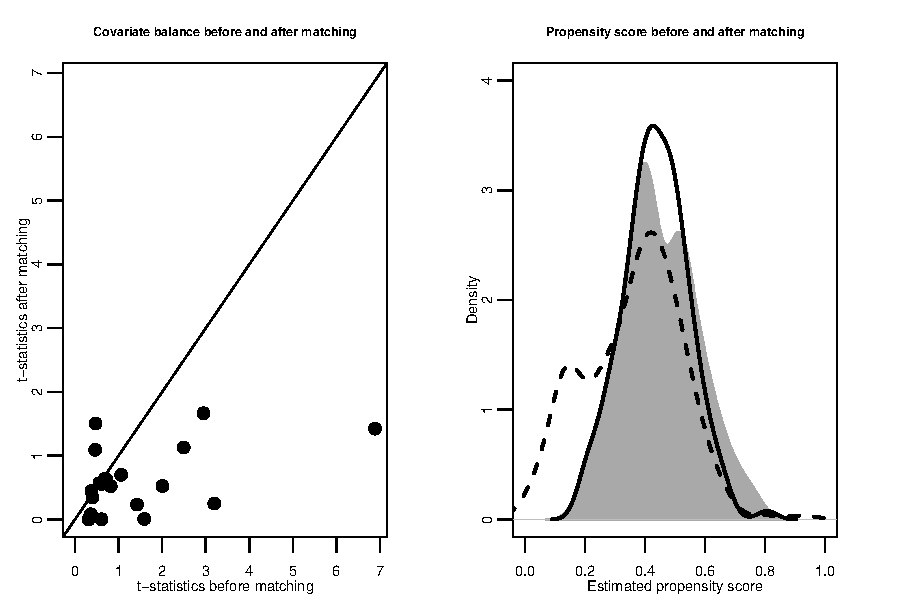
\includegraphics{figs/fdabal.pdf}
  \end{center}
  \vspace{-0.275in}
  \caption{Covariate balance before and after matching for the FDA data.
    The left panel plots the absolute value of t-statistics before and
    after matching for mean differences of each covariate between the
    treatment and control groups. The gray rectangular represents the
    region where t-statistics are not significant at 5\% level for
    both before and after matching. After matching, all t-statistics
    become insignificant. The right panel presents the density plot
    for estimated propensity score before and after matching. After
    matching, the distribution for the control group becomes
    substantially more similar to that for the treatment group.}
  \label{fg:fdabal}
\end{figure}

The right panel of Figure~\ref{fg:fdabal} provides another view of how
our preprocessing improves covariate balance.  Before matching, a
number of control units (drugs) with low values of the propensity
score look very different from the units in the treated group.  The
problem with parametric models applied to raw data is that these
control units will be most influential in any model fit to the raw
data set.  By choosing the matched set of control units which look
most similar to the treated units, the treated-control comparison will
then take place only among units on the background variables and thus
will not be affected as much by the model specification.

We now run the same log-normal survival analysis as Carpenter did, but
using the preprocessed data set.  Since nothing changed other than the
removal of data that would have required highly model-dependent
inferences, no other analysis procedures change.  We compute point
estimates, standard errors, and confidence intervals using the same
procedures Carpenter did on the raw data.  By applying this procedure
to the preprocessed data, the estimated average treatment effect is
$-31.6$ months with an estimated standard error $10.3$, indicating
that a Democratic Senate majority significantly decreases the average
approval time of new drugs.  This result thus continues to contradict
Carpenter's initial hypothesis.

Although data analysis would end here for those interested in the
substantive research questions, for our methodological purposes we go
a step further to demonstrate the model-dependence of the average
causal effect of a Democratic Senate majority using the preprocessed
data and compare this with that from the raw data.  For simplicity, we
portray model dependence by the variability in ATE point estimates
across potential specifications of pretreatment covariates, although
the same conclusions apply to most other quantities of interest too.

We estimate the point estimate of the ATE for every possible
specifications in which the 18 covariates enter the model with the
treatment indicator (i.e., all possible subsets of covariates from the
18).  Even though we ignored interactions and nonlinearities, this
amounts to $262,143$ survival analyses, all of which we ran.
Figure~\ref{fg:fdadens} presents a histogram for the estimated average
treatment effects across all the specifications for the raw data as
well as for the matched (preprocessed) data.  The key result here is
that estimates are far more model-dependent using the raw data than
using the matched data.  For example, the variance of the estimated
average treatment effect from the matched data (the solid curve) is
more than three times as large as that from the raw data (the dashed
curve).  (The distribution of estimates for the matched data is also
closer to the normal density, which will happen when control variables
included are having effects only due to random errors.)
\begin{figure}[t] 
 \begin{center}
   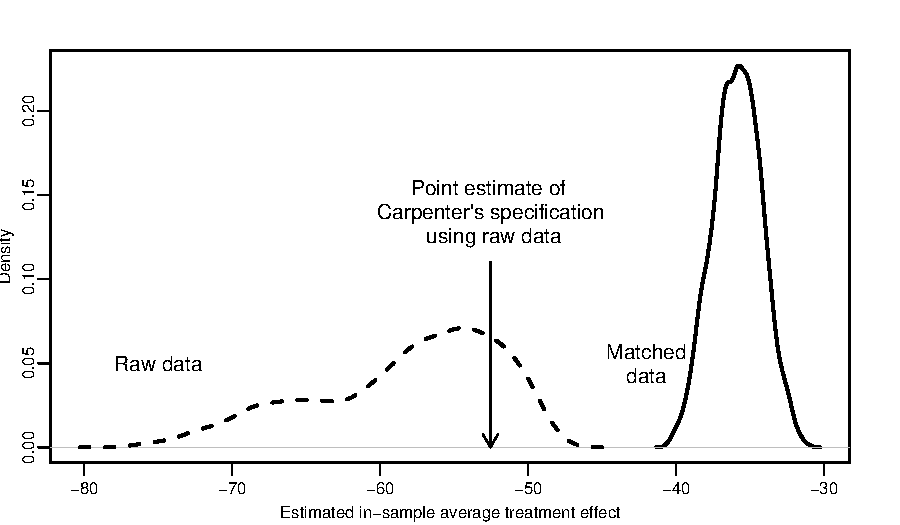
\includegraphics{figs/fdadens.pdf}
  \end{center}
  \vspace{-0.275in}
  \caption{Kernel density plot (a smoothed histogram)
    of the estimated average treatment effect of the Democratic Senate
    majority on FDA drug approval time across $262,143$
    specifications. The solid line presents a density plot of the
    estimated average treatment effect for the matched dataset, while
    the dashed line is for the raw data.  The vertical arrow shows the
    point estimate of the lognormal survival regression from the raw
    data.  The figure shows that average treatment effect estimates
    are considerably more sensitive to model specification using the
    raw data as compared with the preprocessed matched data.}
  \label{fg:fdadens}
\end{figure}

In his original analysis, Carpenter was unable to draw conclusions
from the raw data due to high levels of model dependence. This can be
seen by the density graph with a heavy lower tail in our figure.
However, our preprocessing shows that there does exist sufficient
information in the data to draw conclusions without
difficult-to-justify functional form assumptions.  Contrary to the
original hypothesis, a Democratic Senate majority reduces the average
approval time of new drugs.  Using the raw data, Carpenter notes the
large model sensitivity, concluding that oversight covariates appear
not to matter.  However, the result from the matched data seems to
indicate that the actual effect size may even be larger and more firm
than indicated by the usual parametric approach.

\subsection{Causal Effect of Visibility on Candidate
  Evaluations}

For our second application, we reanalyze a study of citizen
evaluations of the ideological positions of candidates for the U.S.\ 
House of Representatives by \citet{Koch02}.  The quantity of interest
is the causal effect of being a highly visible female candidate on
citizen voter evaluations of the candidate's ideology (scored as a
seven point ordinal scale, where high scores indicate greater
conservatism).\footnote{Visibility is measured originally by whether a
  candidate had campaign expenditures exceeding more than \$750,000.
  For simplicity and comparison to \citet{Koch02}, we stipulate to,
  rather than evaluate the appropriateness of, these measurements or
  methods.}  We confine ourselves to studying this effect on
Republican female candidates, compared to the control of invisible
male and female candidates (corresponding to the fourth column of
Table 2 in \citet[p.  459]{Koch02}).  We begin by replicating the
analysis, which we did successfully.

Since randomly assigning visibility to candidates in real elections is
infeasible, \citet{Koch02} collects observational data with
pretreatment covariates including candidate ideology, voter perception
of party ideology, respondent ideology, candidate feeling thermometer,
and political awareness.  Koch uses least squares to adjust for these
explanatory variables.  We begin with a brief assessment of the
assumptions common to a traditional parametric approach and our
preprocessing approach.  First, the study assumes that visibility does
not itself affect any of the pretreatment covariates.  This might be
violated, for example, if visibility influences the affect felt for a
candidate as measured by the feeling thermometer.  Controlling for the
feeling thermometer would thereby induce post-treatment bias.  Second,
the study assumes that the visibility of one candidate does not affect
the potential outcomes of another candidate.  Visibility of a
candidates might, for example, detract local media attention from a
candidate in an adjoining district, violating independence.  Third,
the study assumes that visibility is the same treatment for all
candidates.

Here, we do not take issue with these three assumptions.  Instead, we
focus on the sensitivity of inferences to differents in specification.
Even with a relatively small number of covariates, the curse of
dimensionality looms large.  Given the combinations that can be
created by the unique values of these covariates and the treatment, it
is easy to calculate that a parametric model that imposes no
unverified functional form assumptions would require estimating
87,530,856 parameters --- a problem of course in a data set with only
494 observations.  Koch reduces these parameters to only six (main
effects) by assuming no interactions or nonlinearities.

The linear adjustments are important since, as the raw data in
Table~\ref{tb:kochmtest} demonstrate, visible and invisible candidates
differ drastically in terms of background explanatory covariates.
Most strikingly, visible female candidates tend to be substantially
more liberal than invisible candidates: visible candidates are rated
0.44 on a scale from 0 to 1, which is almost an entire standard
deviation higher than the 0.2 average rating of invisible candidates
(t-statistic=12.18).  In addition, visible candidates appear to be
slightly more politically aware (t-statistic=2.42).  Extrapolation is
therefore likely to be a significant problem.
\begin{table}[t]
  \begin{center}
    \begin{tabular}{lrrrrrr}
      \hline
      & \MC{3}{c}{} & \MC{3}{c}{\bf Preprocessed Data}\\
      & \MC{3}{c}{\bf Raw Data} & \MC{3}{c}{\bf (subclass 4)}\\
      & Mean for  & Mean for  &    & Mean for  & Mean for \\
      & Treated & Control  & t-stat &    Treated & Control  & t-stat \\
      \hline
      Propensity Score & 0.48 & 0.10 & 10.71 & 0.61 & 0.54 & 2.32 \\
      Candidate Ideology & 0.44 & 0.20 & 12.18 & 0.50 & 0.48 & 1.15 \\
      Perception of Party Ideology & 0.72 & 0.73 & -0.42 & 0.69 & 0.67 & 0.24 \\
      Respondent Ideology & 0.49 & 0.53 & -0.97 & 0.45 & 0.50 & -0.38 \\
      Respondent Ideology $\times$ \\
\hspace{0.1in} Feeling Thermometer  & 0.31 & 0.32 & -0.44 & 0.27 & 0.25 & 0.18\\
      Feeling Thermometer & 0.60 & 0.55 & 1.70 & 0.54 & 0.53 & 0.03 \\
      Political Awareness & 0.76 & 0.70 & 2.42 & 0.76 & 0.74 & 0.28 \\
      \hline
    \end{tabular}
    \caption{Imbalance of pretreatment covariates in Koch data.
      The full sample size is 494, and the preprocessed data size is
      463.  The first three columns present means for visible female
      (``treated'') and invisible (``control'') Republican candidates,
      and t-statistics for the full dataset.  The last three columns
      present means and t-statistics for one representative subclass.
      This table shows that candidate ideology is highly imbalanced in
      the full Koch data, and that balance can be achieved by
      subclassification.  Visible females, for example, were much more
      likely to be perceived as liberal than invisible candidates
      overall, but within subclass 4 this difference diminishes.}
    \label{tb:kochmtest}
  \end{center}
\end{table}

Through experimentation, we find that propensity score matching does
not improve balance much, no matter how we specify the propensity
score equation.  However, subclassifying on the propensity score
improves balance considerably without reducing the number of
observations much, and so we use it.  Our propensity score analysis
involves a logistic regression of visibility on all six pretreatment
covariates.  We also discard treatment units whose propensity score is
greater than the maximum of control units and control units whose
propensity score is lower than the minimum of the treated units.  This
results in 31 discarded units, and (as in Figure \ref{fg:extrap})
greatly reduces the risks of extrapolation.  Next, we create six
subclasses by quantiles of the propensity score of the treated units.
As is desired, covariate balance is substantially better within each
subclass than in the raw data; within each subclass, any extrapolation
would be confined to a region much closer to the data.  For example,
the last three columns of Table~\ref{tb:kochmtest} present means and
t-statistics for each covariate in one representative subclass showing
that balance uniformly increases in each of these covariates.
Candidate ideology, which was highly imbalanced in the raw data, now
has a t-statistic for the difference of only 0.5 for visible
candidates within subclass 4, which differs only slightly from the
0.48 for invisible candidates in that subclass (t-statistic=1.15).

To check balance for all the subclasses, Table~\ref{tb:kochxsub}
presents test statistics for the difference in means for each of the
main covariates, in each of the subclasses.  The last three rows
present the number of units in each subclass.  The preprocessing
procedure matches a small number of visible candidates with many more
invisible candidates in the lower subclasses and the reverse in the
higher subclasses.  This is another indication that in the raw data,
the covariates are highly unbalanced.  Through this simple technique
we are able to compare the most similar candidates within each
subclass.  Indeed, the t-statistics for the difference in covariates
for all subclasses exceed 2 only once, which is roughly the same as we
would expect if treatment were assigned randomly within each subclass.
\begin{table}[t]
  \begin{center}
    \begin{tabular}{lrrrrrr}
      \hline
      & \MC{6}{c}{\bf Subclass} \\
      Covariate &  1 &  2 &  3 &  4 &  5 &  6 \\
      \hline
      Candidate Ideology & 2.16 & -0.85 & 0.33 & 1.15 & 1.51 & -0.45 \\
      Party Ideology & -0.65 & -1.05 & 0.59 & 0.24 & 0.06 & 1.53 \\
      Respondent Ideology & 1.45 & -0.73 & 1.08 & -0.38 & -1.26 & -1.00 \\
      Respondent Ideology $\times$ & 0.50 & -0.81 & 1.64 & 0.18 &
      -1.44 & -0.42 \\
      \hspace{0.1in} Feeling Thermometer \\
      Feeling Thermometer & -0.03 & 0.33 & 1.61 & 0.03 & -1.34 & 1.08 \\
      Political Awareness & 0.53 & 0.14 & -1.50 & 0.28 & -1.08 & 0.66
      \\ \hline
      Treated $n$& 14 & 13 & 13 & 14 & 13 & 11 \\
      Control $n$& 299 & 30 & 39 & 12 & 3 & 2 \\
      Total $n$  & 313 & 43 & 52 & 26 & 16 & 13 \\
      \hline
    \end{tabular}
    \caption{Means test statistics for six pretreatment covariates.
      Each cell presents the t-statistic for the covariate within each
      subclass.  This table shows that relative balance can be
      achieved within each subclass with only six subclasses.}
    \label{tb:kochxsub}
  \end{center}
\end{table}

With this preprocessed data set we can now run the same least squares
analysis as in \citet{Koch02}.  The only difference is that we run the
analysis by subclass, and average the estimates weighting by the
number of treated candidates in each subclass.  This yields an
estimated average treatment effect of $-0.23$ with an estimated
standard error $0.14$, indicating that female visibility might cause
voters to perceive female candidates as more liberal.

We now turn to our main purpose of evaluating model sensitivity by
studying the variance of causal effect point estimates for 63
(=$\sum_{i=1}^6 {6 \choose i}$) regressions containing all possible
subsets of Koch's six covariates, again for simplicity restricting
ourselves to only permutations of the possible main effects.  For the
matched data set, we run the same specification locally within each
subclass, aggregating the point estimates weighted by the number of
treated units in each subclass.  The result in each case is 63
separate point estimates for the raw and for the preprocessed data.

Figure~\ref{fg:kochdens} presents the results, plotting densities of
estimated average treatment effects for the treated (ATT) from the raw
and preprocessed data.  As expected, the estimated treatment effect
estimates are substantially more variable for the raw data.  Estimated
effects from the raw data (see the solid line) range from $-0.64$ to
$-0.2$, signifying that female visibility causes voters to perceive
candidates as more liberal.  The point estimate from the raw data that
controls for all six covariates, signified by the vertical arrow,
appears conservative compared to this range.  Estimates from the
preprocessed data, however, stand in stark contrast to the estimates
from the raw data.  The variability of coefficient estimates is
substantially smaller, ranging from $-0.31$ to $-0.07$, and the
variance across specifications is more than \emph{six} times smaller
than for the raw data, as shown by the highly peaked density.  Rather
than erring on the conservative side, the reported point estimate now
appears to be substantially larger in substantive effect than we might
expect from the more valid and less model-dependent preprocessed data.
\begin{figure}[t] 
 \begin{center}
   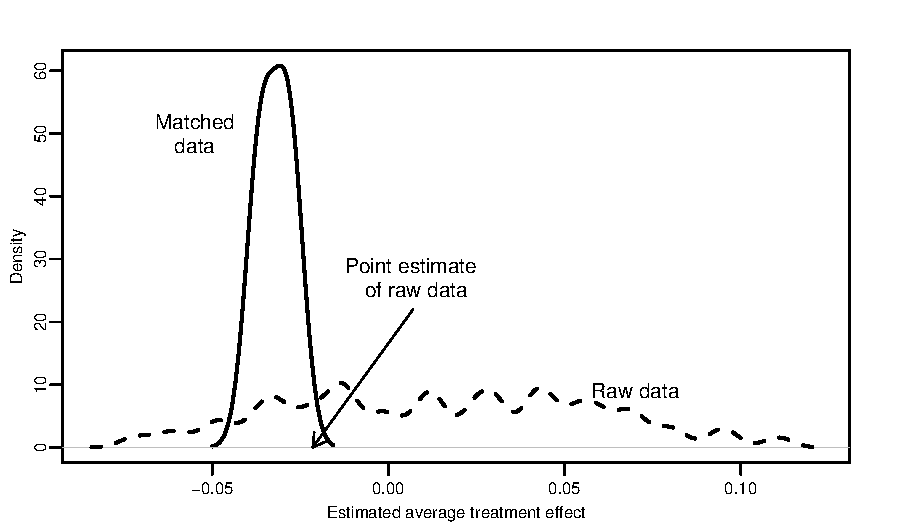
\includegraphics[height=3in,angle=0]{figs/kochdens.pdf}
 \end{center} 
 \vspace{-0.275in}
 \caption{Density estimates of estimated effects of
   being a highly visible female Republican candidate across 63
   possible specifications with the Koch data.  The dashed line
   presents estimates for the raw dataset and the solid line for the
   (subclassified) matched dataset.  The vertical arrow presents the
   point estimate of the regression presented in the original paper.
   This figure shows that treatment effect estimates are much more
   sensitive to model specification for the raw dataset compared to
   the matched dataset.}
 \label{fg:kochdens}
\end{figure}

In short, not only can preprocessing reduce model dependence,
decreasing the probability that researchers may inadvertently present
innacurate estimates, but preprocessing also may change or reinforce
the substantive conclusions of the research.  The fact that treatment
effects may be substantially smaller may even further bolster the
claim that ``[t]he contradictory nature of . . .  [the] cues received
from Republican female candidates presents citizens with a complicated
information-processing task'' \citep[p.  460]{Koch02}.

\section{What Can Go Wrong}

The advantage of matching is that it is relatively robust to small
changes in procedures, and produces a data set that is by design less
sensitive to modeling assumptions.  However, like any method, using it
badly or to ill effect is certainly possible.  Thus, in this section,
we discuss four ways in which preprocessing can go wrong and how
researchers might try to avoid these problems.

First, since the curse of dimensionality affects balancing
diagnostics, we may well miss a higher dimensional aspect of imbalance
when checking lower dimensional summaries.  Even if we are
uninterested in testing these with our parametric model, they can
affect our estimates.  Such will be the case with parametric models
with or without preprocessing, and so in all but the most unusual
cases at least preprocessing should not hurt.  One pathological case
where preprocessing could hurt is if some covariate has a huge effect
on the outcome variable and preprocessing slightly reduces balance on
this variable but improves it for all the others.  A researcher might
be fooled into choosing a matching tradeoff like this if he or she
were not aware of the large effect of this covariate.

Second, as with all statistical methods, a bias-variance tradeoff
exists for matching.  If we drop many observations during
preprocessing and balance is not substantially improved, the mean
square error (or other mean-variance summary) might actually increase.
Users must pay close attention to this tradeoff during the process of
matching, but no precise rules exist for how to make these choices.
In particular, the methodological literature offers no formal
estimates of mean square error and so in marginal cases it can be
difficult to know whether or how much preprocessing will help.  Of
course, dropping many observations does not necessarily mean that
preprocessing is worse, since including imbalanced observations in a
parametric analysis merely produces false precision.  So although
estimated standard errors may increase in some cases with
preprocessing, they would be more accurate.  Moreover, in many
situations, eliminating observations far from the data as matching
does will sometimes reduce heterogeneity and thereby reduce the
variance.

Third, the matching literature offers a large number of possible and
seemingly ad hoc procedures.  From one perspective, we might be
concerned about the sensitivity of our results to changes in this
process, just as we have been concerned with the sensitivity of causal
effect estimates to parametric modeling assumptions.  In our view,
this is not a major issue since the right procedure is the one that
maximizes balance (with an as large as possible $n$), no matter how
many procedures we try.  By applying this criterion in a disciplined
way (i.e., without consulting $y$) to a large number of possible
matching procedures, no choices are open to the analyst.  Instead,
researchers should merely run as many as possible and choose by this
relatively automatic procedure.  Unlike parametric modeling exercises,
we need not choose this matching procedure or another; we merely run
as many as feasible or likely to reduce bias and apply this criterion.

Finally, by dropping observations, we may wind up losing some
critically important cases or may change either the information base
of our sample or, in special cases such as when dropping treated
units, the definition of causal effect.  Examining the dropped cases
provides an easy diagnostic for this problem.  However, we must be
alert to the problem that if we learn that some critical units are
dropped, then it may mean that no appropriate matches can be found for
them.  In this situation, we may be forced to conclude that the data
do not contain sufficient information to answer the questions posed,
no matter what method is chosen.

\section{Concluding Remarks}

Anyone using a parametric statistical technique for long enough (and
it doesn't take very long) will recognize the difficulty of choosing
which of hundreds of possible regressions to present in a written
work.  This choice is difficult, fraught with ethical and
methodological dilemmas, and not covered in any serious way in
classical statistics texts.  Parametric methods merely assume that we
know the correct specification.  In practice, the ``correct''
specification is chosen after looking at the estimates and so it is
never clear to a reader whether an article is a true test of an ex
ante hypothesis, in the sense that the author was vulnerable to being
proved wrong, or whether the article is merely a proof that it is
\emph{possible} to find a specification consistent with the author's
favored hypothesis.

We provide a way around at least part of this problem.  Preprocessing
raw data with the matching procedures we recommend makes familiar
parametric methods a much more reliable tool of empirical analysis,
and in particular, causal effect estimates become far more insensitive
to seemingly arbitrary choices in model specification.  If we read an
article demonstrating that balance has been achieved for a data set,
readers need not worry that slightly different specifications than
those discussed in the text will greatly alter its empirical
conclusions.

\appendix
\section{Matching Software}\label{s:matchit}

We have created a software package called MatchIt (available at
\url{http://gking.harvard.edu/matchit/}) that implements a large
fraction of the matching procedures suggested in the diverse scholarly
literatures on this subject.  Most of our software operates with a
single command that takes an existing dataset and produces as output a
single preprocessed matched dataset.  The preprocessed matched dataset
can then be used by standard parametric software just as you would
have used the original dataset.  MatchIt also works seemlessly with
the general-purpose statistics program, Zelig (\citet{ImaKinLau04},
available at \url{http://gking.harvard.edu/zelig}).  MatchIt and Zelig
run under most operating systems via the open-source statistical
program R (see \url{http://r-project.org}).  MatchIt, Zelig, and R are
available free of charge.

For example, to use propensity score matching of a treatment
indicator, \texttt{treat}, and three pretreatment covariates, use this
command:
\begin{verbatim}
match.out <- matchit(treat ~ age + educ + black, data = koch)
\end{verbatim}
with the output stored as \texttt{match.out}.  For exact matching use:
\begin{verbatim}
match.out <- matchit(treat ~ age + educ + black, exact=TRUE, data = carpenter)
\end{verbatim}
Numerous other options are also available.

Suppose we use MatchIt to subclassify into 5 classes by the propensity
score:
\begin{verbatim}
match.out <- matchit(treat ~ age + educ + black, subclass=5, data = koch)
\end{verbatim}
Then we can easily use Zelig to estimate a parametric model (in this
case least squares regression) within each of the five subclasses
defined in MatchIt, using data from the control group:
\begin{verbatim}
z.out <- zelig(re78 ~ pscore, model = "ls", by = "psclass", 
                data = match.data(match.out, "control"))
\end{verbatim}
With Zelig, we can also set the explanatory variables to predict the
missing potential outcomes under control for the treatment group and
simulate quantities of interest within each subclass:
\begin{verbatim}
x.out <- setx(z.out, data = match.data(match.out, "treat"), cond = TRUE)
s.out <- sim(z.out, x = x.out)
\end{verbatim}
The output automatically weights the results by the separate subclasses.
\baselineskip=0.637\baselineskip \bibliographystyle{apsr}
\bibliography{gk,gkpubs}

\end{document}
